\documentclass[11pt]{article}
\usepackage[margin=1in]{geometry}
\usepackage{amsmath,amssymb}
\usepackage{graphicx}
\usepackage{booktabs}
\usepackage[numbers]{natbib}
\usepackage[colorlinks=true,allcolors=blue]{hyperref}

\title{A Descriptive Title of Your Study}
\author{First Author\thanks{Department, University, \texttt{first@example.edu}}
  \and Second Author}
\date{\today}

\begin{document}
\maketitle

\begin{abstract}
State the problem, what you did, the main result and why it matters, in about 150 words.
\end{abstract}

\section{Introduction}
\label{sec:intro}
Introduce the background and the gap your work fills~\citep{knuth1984,lamport1994}.
Section~\ref{sec:method} describes the method and Section~\ref{sec:results} the results.

\section{Method}
\label{sec:method}
Define the quantities you use. For example, the free energy
\begin{equation}
  \label{eq:energy}
  G = H - TS
\end{equation}
relates the enthalpy $H$, the temperature $T$ and the entropy $S$.

\section{Results}
\label{sec:results}
Figure~\ref{fig:example} and Table~\ref{tab:example} summarise the results.

\begin{figure}[ht]
  \centering
  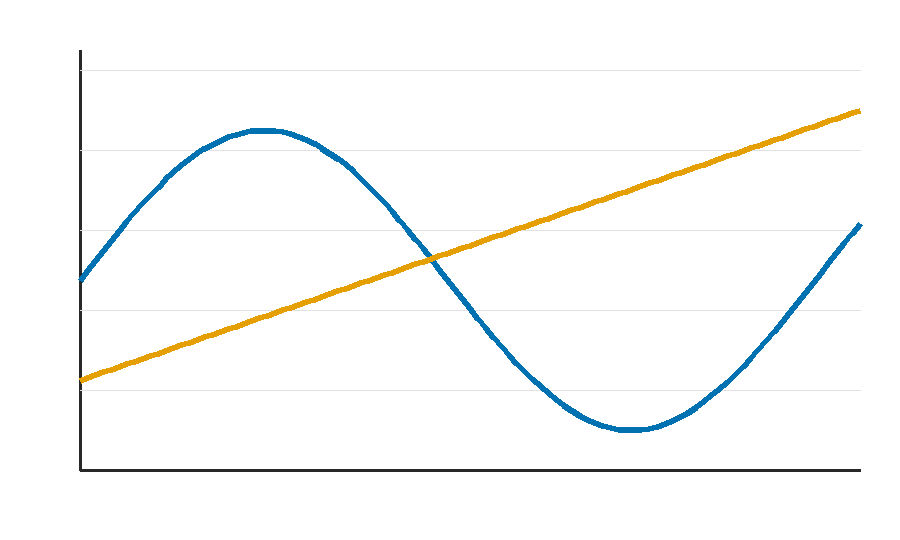
\includegraphics[width=0.6\linewidth]{figures/example.png}
  \caption{Replace this figure with your own; keep figures in the \texttt{figures} folder.}
  \label{fig:example}
\end{figure}

\begin{table}[ht]
  \centering
  \caption{An example table.}
  \label{tab:example}
  \begin{tabular}{lcc}
    \toprule
    Sample & Value A & Value B \\
    \midrule
    S1 & 1.00 & 2.00 \\
    S2 & 1.50 & 2.50 \\
    \bottomrule
  \end{tabular}
\end{table}

\section{Conclusion}
Summarise the findings and the next steps.

\bibliographystyle{plainnat}
\bibliography{refs}

\end{document}
